\section{Introduction}
\label{sec:Introduction}

Machine learning force fields (MLFF) provide a computationally efficient and low-cost approach to learning the interactions between atoms, bringing revolutionary advances to molecular dynamics simulations across physics, chemistry, biology, and materials science~\cite{behler2007generalized,unke2021machine,chmiela2017machine,xiang2024molecular,wang2024efficiently}. However, current MLFF methods, built on geometric deep learning with E(3)-equivariant architectures~\cite{thomas2018tensor,fuchs2020se3,liu2022spherical,wang2024enhancing}, focus on atom-level physical quantities such as coordinates and multi-body interactions~\cite{batzner20223,liao2023equiformer,wang2024enhancing}, while ignoring information at the electronic level.

Electron density (ED) describes the probability density of finding an electron at a given point in three-dimensional space and is a foundational quantity for predicting the quantum chemical properties of MFF~\cite{sunshine2023chemical,skogh2024electron}. The Hohenberg-Kohn theorem~\cite{hohenberg1964inhomogeneous} formalizes this relationship by establishing that the ground-state energy is a unique functional of the electron density. Despite this central role, exploiting ED in MLFF faces three major challenges:

\begin{figure*}[htbp]
\centering
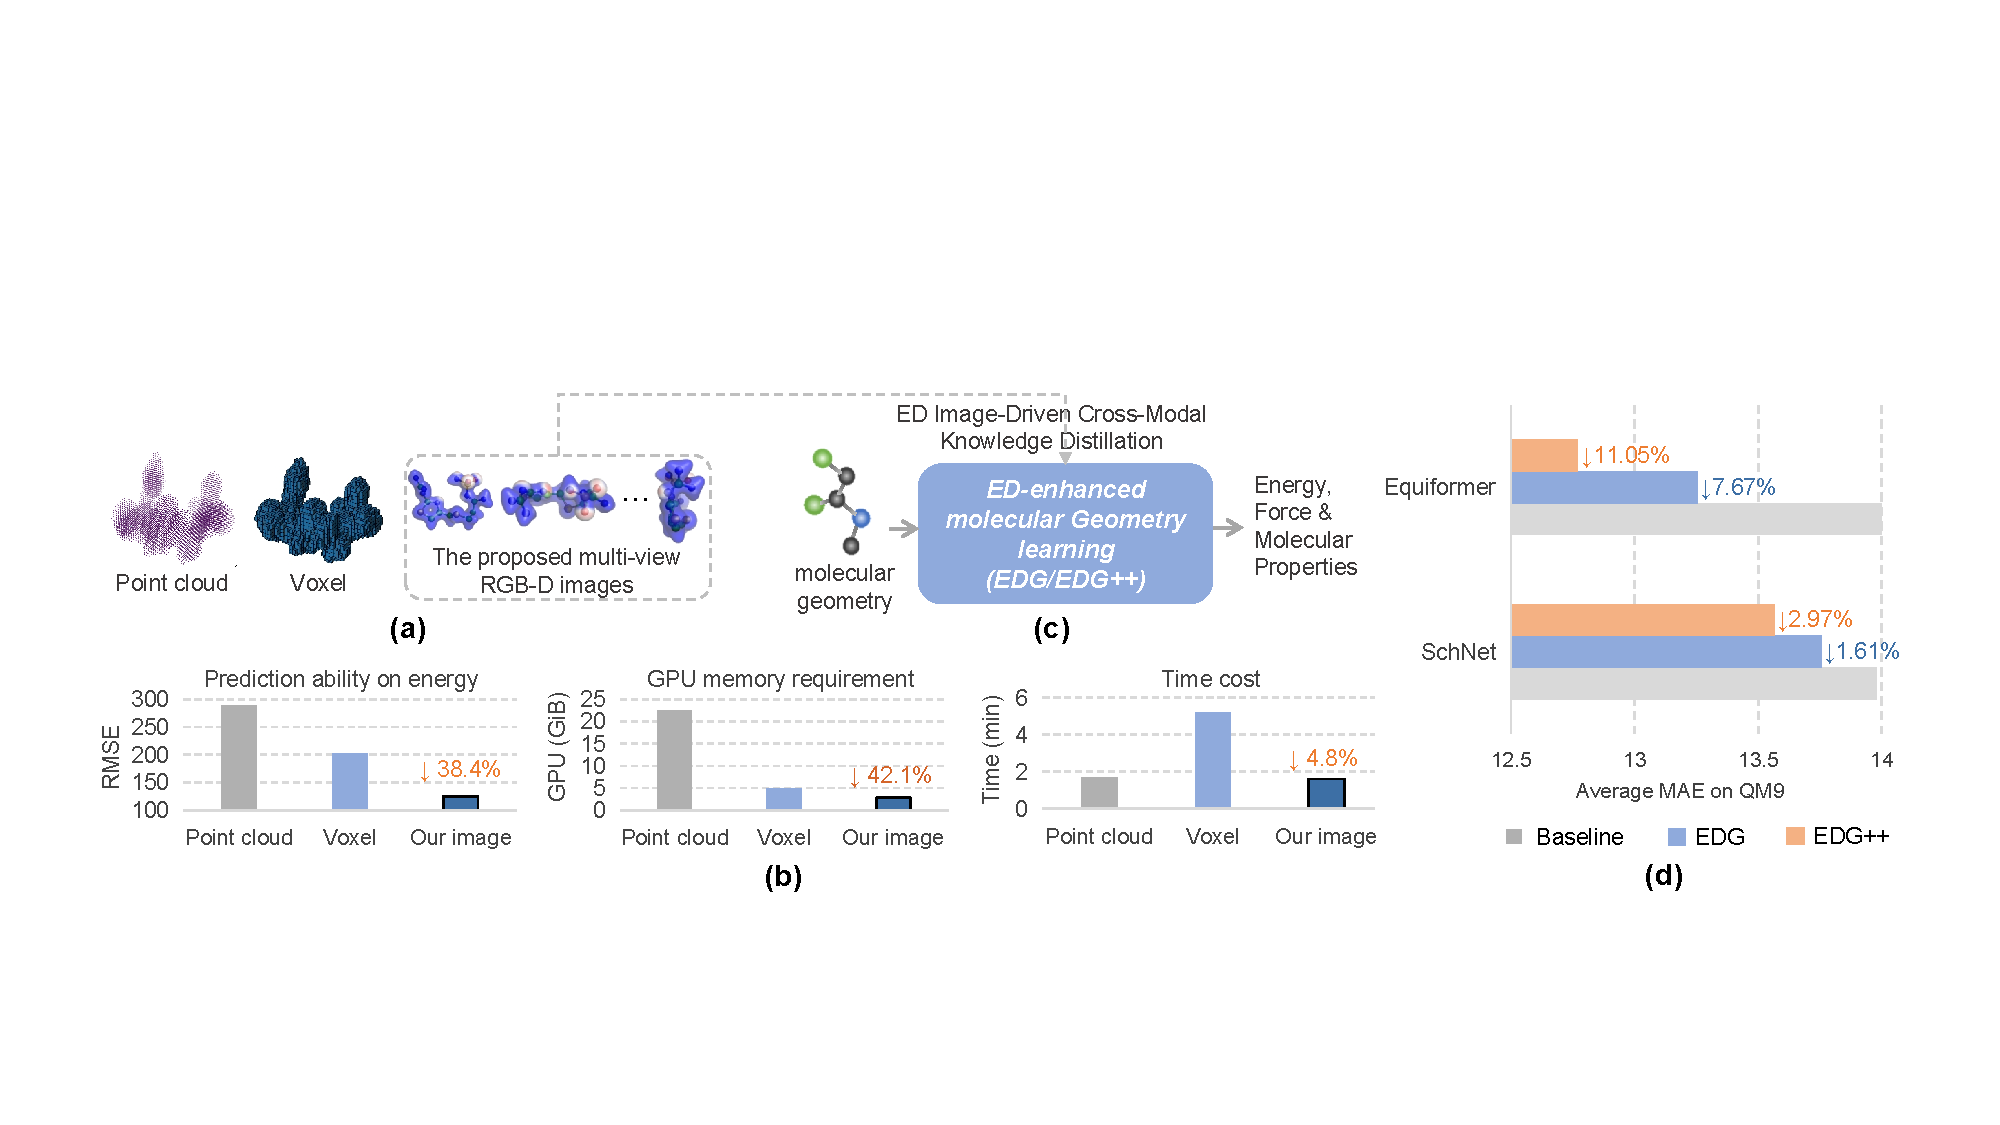
\includegraphics[width=\textwidth]{imgs_edgpp/introduction/fig1_introduction.pdf}
\caption{Motivation and overview (detailed pipeline in Fig.~\ref{Fig2_Method}). (a) ED representation methods. (b) RMSE, GPU memory, and training time of different ED representations. (c) High-level EDG/EDG++ framework: multi-view ED images with RGB-D channels enhance molecular geometry learning; EDG++ adds reliability-aware selective distillation. (d) Average MAE on 12 QM9 tasks. EDG improves both SchNet and Equiformer; EDG++ further improves through reliability-aware selective distillation.}
\label{Fig1_Intro}
\end{figure*}

% [Polish] Original: \textit{Challenge 1: High computational complexity of ED.} Unlike the number of atoms in a molecule, which is usually on the scale of tens to hundreds, the ED relies on a continuous spatial distribution and as the resolution increases, the number of data points may reach millions or even tens of millions. As shown in Fig.~\ref{Fig1_Intro}(a), there are two direct ways to represent ED: point cloud~\cite{guo2020deep} and voxel~\cite{gong2023incorporation}. As shown in Fig.~\ref{Fig1_Intro}(b), we empirically show the limitations of point clouds and voxels as ED representations in energy prediction, GPU memory efficiency, and training efficiency. In particular, point clouds and voxels are directly related to the resolution of the ED, so the computational efficiency will decrease as the resolution increases. These limitations motivate us to propose a multi-view RGB-D image (the right subfigure of Fig.~\ref{Fig1_Intro}(a)) for accurate and efficient ED representation, which produces a fixed-size output regardless of ED grid resolution and compresses the continuous ED signal into pixels. Compared with point clouds and voxels, the proposed images improve energy prediction ability, GPU memory efficiency, and training efficiency by 38.4\%, 42.1\%, and 4.8\%, respectively.
\textit{Challenge 1: High computational complexity of ED.} ED is defined on a continuous spatial domain, with grid points reaching millions or tens of millions as resolution increases---far larger than the tens-to-hundreds scale of atomic nodes. As shown in Fig.~\ref{Fig1_Intro}(a), existing approaches represent ED as either point clouds~\cite{guo2020deep} or voxels~\cite{gong2023incorporation}, both suffering from two limitations: (1)~limited energy-prediction accuracy due to information loss in discretization (Fig.~\ref{Fig1_Intro}(b)); (2)~GPU memory and training cost that scale directly with ED resolution. To address both limitations, we propose a multi-view RGB-D image representation (right subfigure of Fig.~\ref{Fig1_Intro}(a)) that produces a fixed-size output independent of ED grid resolution and compresses the continuous ED signal into pixels. Compared with point clouds and voxels, our representation improves energy prediction, GPU memory efficiency, and training efficiency by 38.4\%, 42.1\%, and 4.8\%, respectively.

\textit{Challenge 2: Expensive ED acquisition.} Obtaining ground-state ED at the level required by MFF relies on computationally intensive quantum chemical calculations such as density functional theory (DFT)~\cite{kohn1965self,hegde2017machine,lee2024convolutional}, which demand substantial computing resources and become prohibitive at scale. As shown in Fig.~\ref{Fig1_Intro}(c), we recast ED-enhanced geometry learning as a teacher-student paradigm: we first use DFT to compute 2 million high-quality ED examples and pre-train an ED representation learning model (ImageED); we then transfer this knowledge to an ED-aware teacher that takes ED-free structural images as input, which subsequently distills geometry students. This scheme, called \textbf{EDG} (Electron Density-enhanced Geometry learning), requires ED computation only once during pre-training and eliminates the need for ED data in all downstream stages. As shown in Fig.~\ref{Fig1_Intro}(d), geometry students equipped with EDG achieve consistent improvements on QM9. However, this naive scheme treats all teacher predictions equally, which motivates the third challenge below.

\textit{Challenge 3: Unreliable teacher predictions causing negative transfer.} Beyond feasibility and efficiency, a critical question remains: \emph{when should we trust the teacher's predictions?} The quality of cross-modal predictions varies across samples due to intrinsic DFT approximations, molecular conformation diversity, and information loss when compressing 3D electron clouds into 2D images. \emph{Naive distillation implicitly assumes uniform teacher fidelity, risking negative transfer}~\cite{pan2010survey}. To address this, we propose \textbf{EDG++}, a reliability-aware extension that introduces a pre-trained reliability estimator and an adaptive global-local thresholding mechanism for selective distillation, filtering unreliable teacher predictions before knowledge transfer (Section~\ref{sec:Theoretical_Analysis}--\ref{sec:Adaptive_Thresholding}). Equipped with this mechanism, EDG++ achieves consistent improvements on 34/36 QM9 task-model combinations and 55/60 rMD17 energy/force tasks, with up to 27--38\% tail-error reduction on the hardest 1\% of samples.

We summarize the main contributions as follows:
\begin{itemize}[itemsep=2pt,topsep=0pt,parsep=0pt]
    \item We propose multi-view RGB-D images as an efficient and resolution-independent representation of electron density, and develop ImageED, a masked autoencoder that learns ED-related features from this representation.
    \item Building on ImageED, we propose EDG, a cross-modal distillation framework that transfers ED knowledge to geometry-based MLFF models through an ED-aware teacher, with no additional computational cost at inference.
    \item We further propose EDG++, integrating a pre-trained reliability estimator with an adaptive global-local thresholding mechanism for selective distillation to mitigate negative transfer.
    \item Extensive experiments validate EDG/EDG++ across diverse student architectures: SchNet, Equiformer, and SphereNet on QM9; SchNet, SphereNet, and ViSNet on rMD17. EDG++ improves on 34/36 QM9 task-model combinations and 55/60 rMD17 energy/force tasks.
    \item We design an out-of-distribution case study on the 166-atom mini-protein Chignolin (Sec.~\ref{sec:case_study_chignolin}), where EDG++'s reliability gating successfully mitigates negative transfer in realistic OOD settings.
\end{itemize}

\textbf{Difference with Conference Version.} Table~\ref{tab:conf_vs_journal} summarizes the key differences between the IJCAI 2025 conference paper~\cite{xiang2025edg} (EDG) and this journal extension (EDG++).

\begin{table}[!htb]
  \centering
  \caption{Conference (IJCAI 2025) vs.\ journal extension.}
  \label{tab:conf_vs_journal}
  \scriptsize
  \setlength{\tabcolsep}{3pt}
  \begin{tabular}{@{}lcc@{}}
    \toprule
    \textbf{Aspect} & \textbf{Conference (EDG)} & \textbf{Journal (EDG++)} \\
    \midrule
    Distillation & Naive (all samples) & Selective (reliability-aware) \\
    Reliability est.\ & -- & Pre-trained; \texttildelow131K params \\
    Thresholding & -- & Adaptive global-local \\
    Architecture cov.\ & EDG only & EDG++ on all three \\
                       &          & students per benchmark \\
    Ablations & $\lambda$ only & $\beta$ (hybrid), $\kappa$ (strictness) \\
    OOD case study & -- & Chignolin (166 atoms) \\
    \bottomrule
  \end{tabular}
\end{table}
